\chapter{General machine learning methods}
In this master thesis, we will use several general machine learning methods in conjunction with each other. In this chapter we will introduce and explain these methods.

\section{Artificial Neural Networks (ANNs)}
In this section we will explain artificial neural networks (ANN). In particular, we will focus on multilayered neural networks (MLNN). We refer to \cite[Chapter 1]{Aggarwal18} and \cite{rong2016word2vec} when describing this section.

\begin{definition}
An artificial neuron (or unit) is a function which receives one or more inputs and a bias, and then sums them to produce an output, as illustrated in \cref{fig:artificial_neuron}; $\left\{ x_1, \ldots, x_K \right\}$ are the input values, $x_0$ is the bias, $\left\{ w_0, \ldots, w_K \right\}$ are the weights and $y$ is a scalar output. We denote $f$ as the activation function.
\end{definition}

\begin{figure}
    \centering
    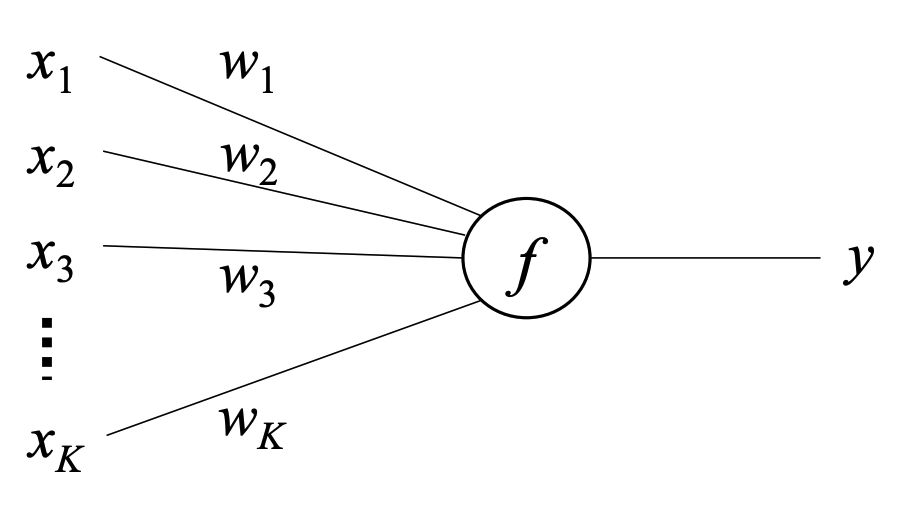
\includegraphics[width=8cm]{thesis/figures/artificial-neuron-rong-2014.png}
    \caption{An artificial neuron as illustrated by \cite[Figure 5]{rong2016word2vec}. Note that the bias is omitted from this illustration (i.e. $x_0=0$).}
    \label{fig:artificial_neuron}
\end{figure}

To produce the output of a single unit, we do the following
\begin{align}
    y = f(u)
\end{align}
where $u$ is the input of the neuron. $u$ is defined as
\begin{align}
    u = \sumlim{i=0}{K} w_i x_i
\end{align}
which is the weighted sum of the input values (including bias term) $\left\{ x_0, \ldots, x_K \right\}$ with $\left\{ w_0, \ldots, w_K \right\}$ as weights.

The bias term acts as a intercept value to make the model more general and is usually set to 1. For some models (e.g. word2vec, introduced in \cref{sec:word2vec-as-an-ann}), one does not include the bias term for the units in the neural network, i.e., we leave $x_0$ to be zero.

The choice of activation function $f$ is typically a non-linear function. Artificial neural networks use different activation functions such as ReLU, sigmoid or tanh to learn non-linear relationships in the data. We will come back to this in \cref{sec:activation-functions-ann}.

\newcommand{\layer}[2]{\left\{ {#1}_{#2} \right\}}

\begin{definition}
\label{def:layer_ann}
A layer $\layer{z}{j} = \left\{ z_1, z_2, \ldots, z_K \right\}$ of an artificial neural network is a collection of artificial neurons (unit). More formally, the layer $\layer{z}{j}$ can be described using an $N \times K$-dimensional weight matrix $W$, a $N$-dimensional bias vector $b$ and an activation function $f$; see \cref{eqn:artificial_layer}.
\end{definition}

\begin{align}
    \layer{z}{j} = f \left( W \cdot x + b \right)
    \label{eqn:artificial_layer}
\end{align}
where $x$ is a $K$-dimensional input vector. Note that we here separate $x$ and $b$ into separate vectors.

In the following subsections, we will go over the different types of layers in the ANN, namely the input, hidden and output layers.

\subsection{Input layer}
\label{sec:ann-input-layer}
The first layer in the ANN is the input layer $\layer{x}{k} = \left\{ x_1, x_2, \ldots, x_K \right\}$. It is responsible for taking in input and passing it to the proceeding layer in the network. We illustrate the input layer in \cref{fig:input_layer_ann}.

\begin{figure}[H]
    \centering
    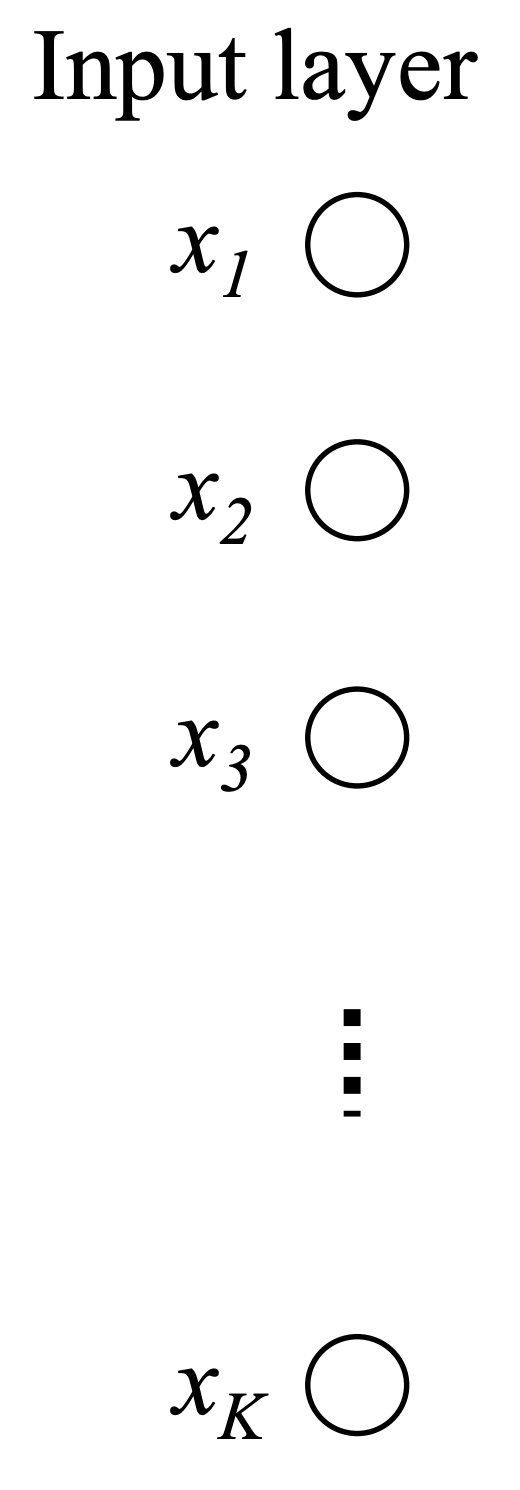
\includegraphics[height=7cm]{thesis/figures/ann-input-layer-rong-2014.png}
    \caption{Input layer in the ANN for a $K$-dimensional vector $x$. The bias $x_0$ is omitted from this figure. Illustration is taken from \cite[Figure 6]{rong2016word2vec}.}
    \label{fig:input_layer_ann}
\end{figure}

More formally, we define the input layer in \cref{eqn:input_layer_ann} using \cref{def:layer_ann}. The layer does not perform any changes to the incoming data and acts as a way for feeding data into the neural network. For this reason, \cref{eqn:input_layer_ann} uses the identity matrix $I_K$ as the weight matrix $W_{\layer{x}{k}}$, the $K$-dimensional bias vector $b_{\layer{x}{k}}$ consisting of all zeros and the identity function $id(x)=x$ as the activation function.
\begin{align}
    \label{eqn:input_layer_ann}
    \layer{x}{k}
    &= f_{\layer{x}{k}}(W_{\layer{x}{k}} \cdot x + b_{\layer{x}{k}}) \\
    &= id(I_K \cdot x) \\
    &= I_K \cdot x \\
    &= x
\end{align}
With this in mind, we look at the layer the input layer is connected to, namely the hidden layer.

\subsection{Hidden layer}
The hidden layer is the second layer in the ANN $\layer{h}{i} = \left\{ h_1, h_2, \ldots, h_N \right\}$, and is most commonly connected to the input layer. It should be noted, however, that we might have multiple hidden layers in the ANN (making the neural network deeper), connecting them to each other. For illustration purposes, we will assume that we only have one hidden layer in our neural network. The hidden layer is illustrated in \cref{fig:hidden_layer_ann}. Here we observe that every unit in the input layer is connected to the units in the hidden layer, as illustrated the lines. This is what we call fully connected layers, meaning that every unit is connected to each other.

\begin{figure}[H]
    \centering
    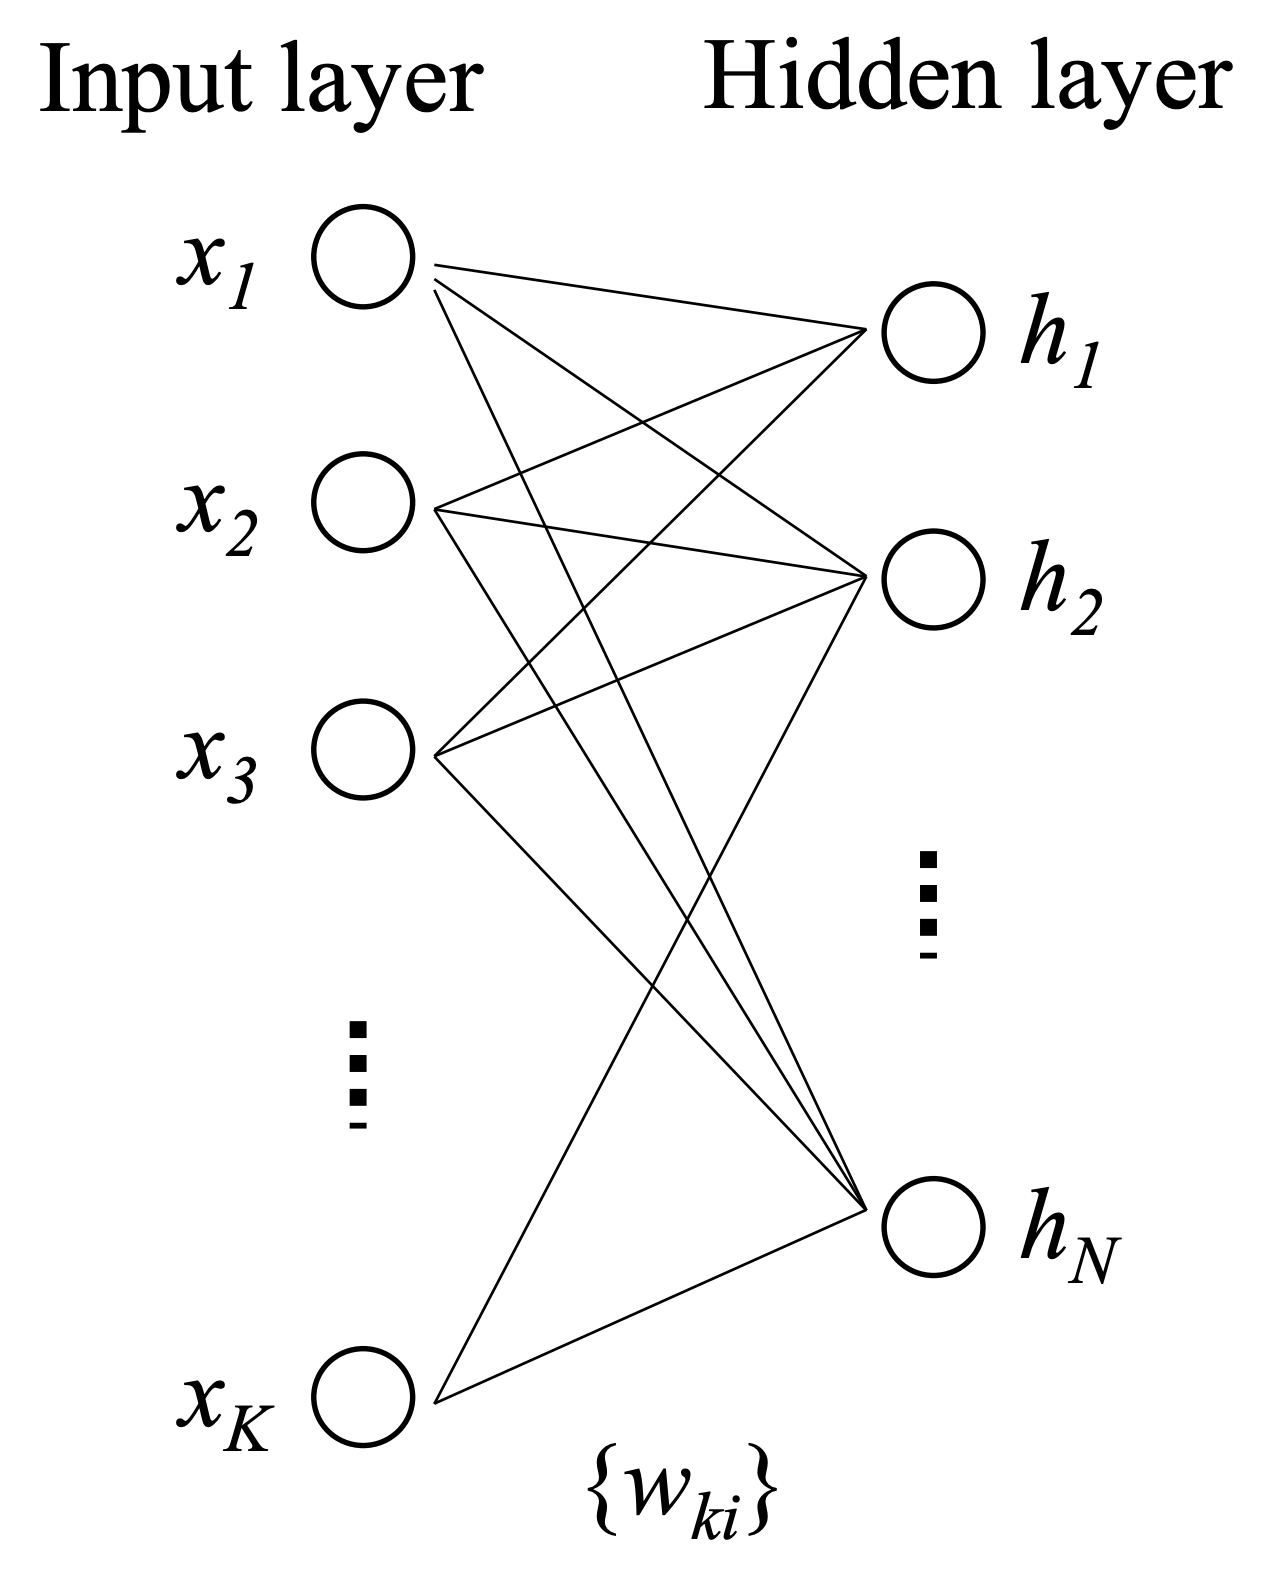
\includegraphics[height=7cm]{thesis/figures/ann-input-hidden-layer-rong-2014.png}
    \caption{Input to hidden layer in the ANN for a $K$-dimensional vector $x$, $N\times K$ dimensional weight matrix $\left\{ w_{ki} \right\}$ and a $N$-dimensional hidden layer $h$. Illustration is taken from \cite[Figure 6]{rong2016word2vec}.}
    \label{fig:hidden_layer_ann}
\end{figure}

We formalize the description of the hidden layer in \cref{eqn:hidden-layer-ann}
\begin{align}
    \label{eqn:hidden-layer-ann}
    \layer{h}{i} &= f_{\layer{h}{i}}(W_{\layer{h}{i}} \cdot \layer{x}{k} + b_{\layer{h}{i}})
\end{align}
where $f_{\layer{h}{i}}$ is a user-specified activation function, $W_{\layer{h}{i}}$ is an $N \times K$-dimensional weight matrix and $b_{\layer{h}{i}}$ is an $N$-dimensional bias vector.

The hidden layer tries to learn a latent representation of the input data $x$. We will explain how the neural network learns the latent representation when introducing optimizers in \cref{sec:optimizers-ann}. Assuming that we have some $N$-dimensional latent representation of the data, we would like to connect it to the final layer in the neural network, namely the output layer.

\subsection{Output layer}
The last layer in the ANN is the output layer $\layer{y}{j} = \left\{ y_1, y_2, \ldots, y_M \right\}$ and is connected to the last hidden layer. Similar to the hidden layer, we connect each unit in the last hidden layer to each unit in the output layer, as illustrated in \cref{fig:mlnn-one-hidden}.

\begin{figure}[H]
    \centering
    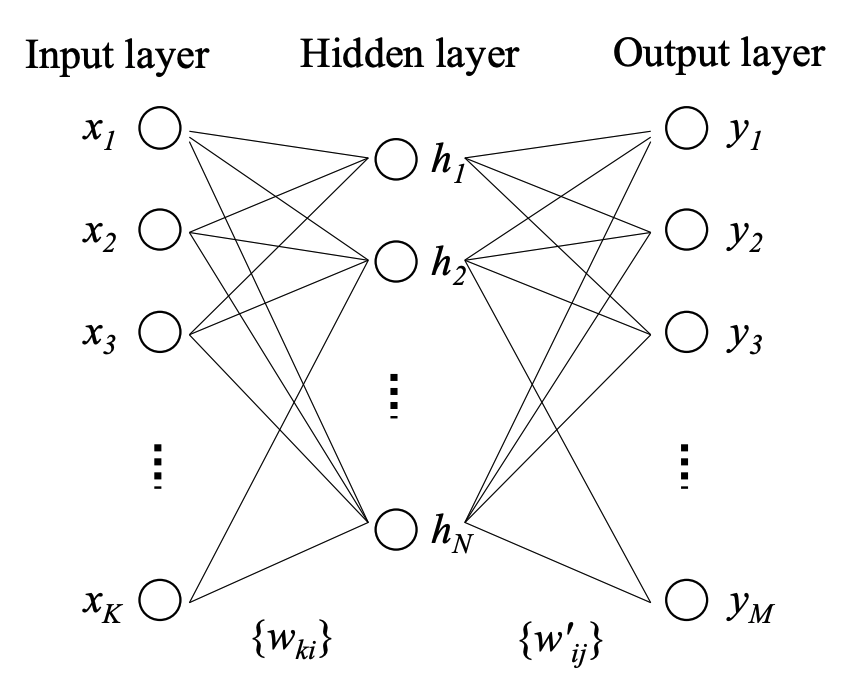
\includegraphics[width=8cm]{thesis/figures/multi-layer-neural-network-one-hidden-rong-2014.png}
    \caption{Multilayered neural network (MLNN) with one hidden layer, as illustrated by \cite[Figure 6]{rong2016word2vec}.}
    \label{fig:mlnn-one-hidden}
\end{figure}

More formally, we define the output layer $\layer{y}{j}$ using a $M \times N$ weight matrix $W_{\layer{y}{j}}$, an $M$-dimensional bias vector $b_{\layer{y}{j}}$ and an activation function $f_{\layer{y}{j}}$, as seen in \cref{eqn:output-layer-ann}.

\begin{align}
    \label{eqn:output-layer-ann}
    \layer{y}{j} &= f_{\layer{y}{j}}(W_{\layer{y}{j}} \cdot \layer{h}{i} + b_{\layer{y}{j}})
\end{align}

We have now covered the different layers in an MLNN, but have yet to cover the different choices of activation function $f$ in the neural network and how the MLNN learns.

\subsection{Activation functions}
\label{sec:activation-functions-ann}
The data which is fed into an ANN might contain complex patterns and have non-linear relationships. To deal with this problem, one applies an activation function to each layer before the result is sent to the proceeding layer. There are several choices of activation functions, and we will go over some of the most common ones.

The simplest type of activation is the identity function, as seen in \cref{eqn:identity-function}.
\begin{align}
    \label{eqn:identity-function}
    f(x) = x
\end{align}

The identity function is commonly used when we want to pass on the values from one layer to another without modifying the value itself, as we have already seen in \cref{sec:ann-input-layer}.

Other choices of activation functions include  sigmoid, tanh, Rectified Linear Unit (ReLU) and softmax, as illustrated in \cref{fig:activation-functions}.
\begin{align}
    \label{eqn:sigmoid-function}
    f(x) &= \frac{1}{1 + \exp{ \left( -x \right) }} \thickspace \text{(sigmoid function)} \\
    \label{eqn:tanh-function}
    f(x) &= \frac{\exp{ \left( 2x \right) } - 1}{\exp{ \left( 2x \right) } + 1} \thickspace \text{(tanh function)} \\
    \label{eqn:relu-function}
    f(x) &= \max{\left\{ x, 0 \right\}} \thickspace \text{(ReLU function)} \\
    \label{eqn:softmax-function}
    f(x_i) &= \frac{\exp \left( x_i \right)}{\sumlim{j=1}{K} \exp \left( x_j \right)} \thickspace \text{, $i \in \left\{ 1, \ldots, K \right\}$ (softmax function)}
\end{align}
where $K$ is the number of output values for the softmax layer.

\begin{figure}[H]
    \centering
    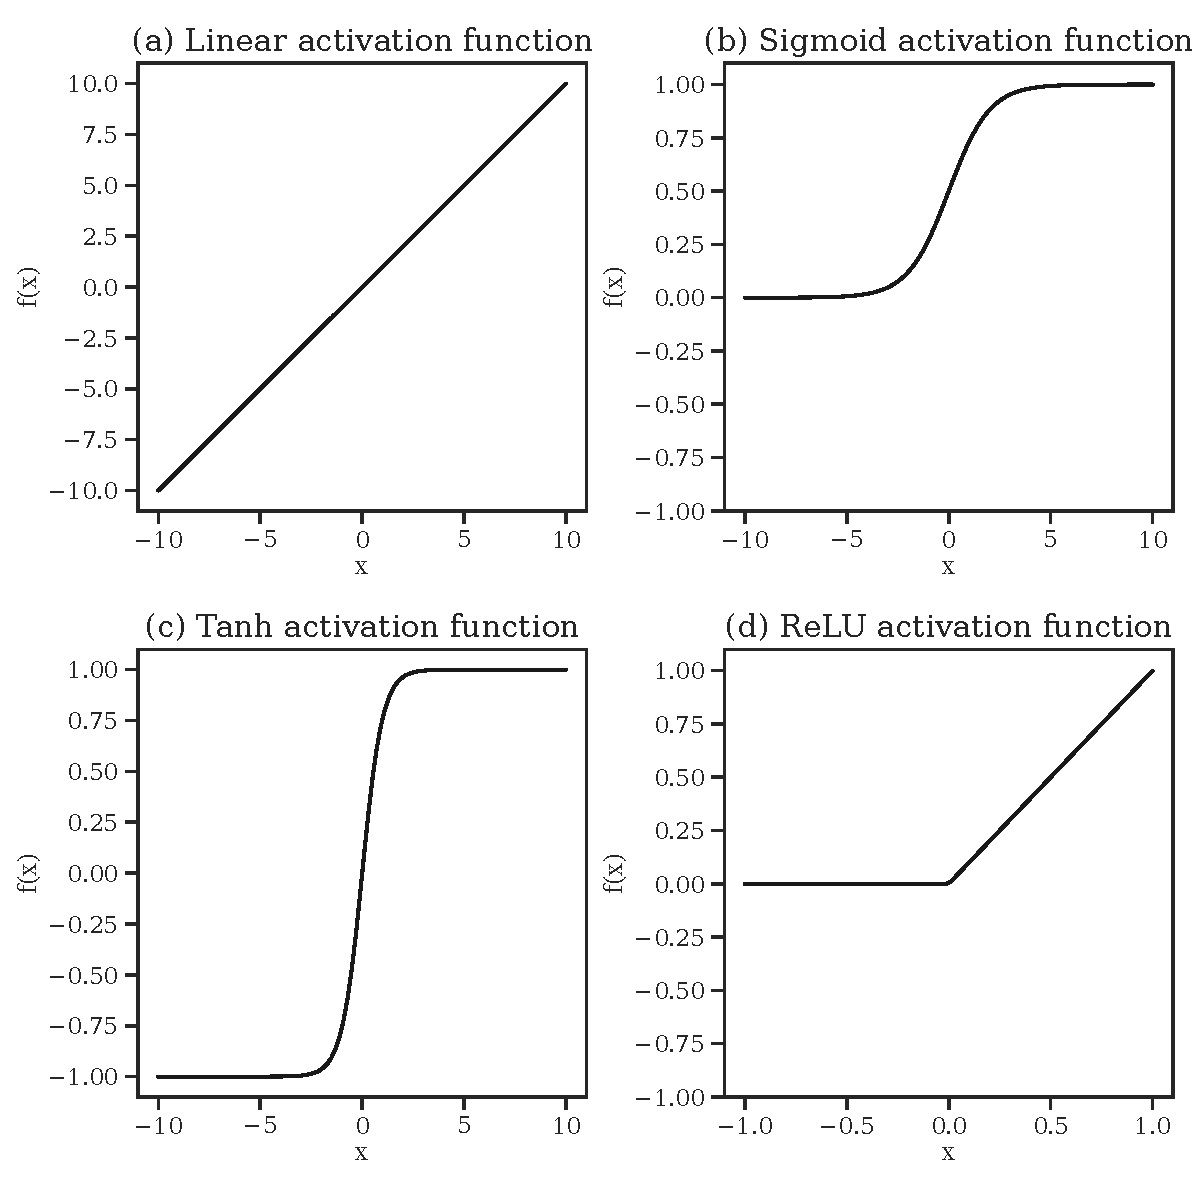
\includegraphics[width=0.7\textwidth]{thesis/figures/common-activation-functions.pdf}
    \caption{Various activation functions}
    \label{fig:activation-functions}
\end{figure}

The sigmoid and tanh activation functions were typically used in the early development of neural networks. The sigmoid activation function maps a value to a value in $(0, 1)$ and is particularly useful since it creates a probabilistic output. The tanh activation function has a similar shape to the sigmoid activation function, and maps values to values in $[-1, 1]$. In fact, the tanh and sigmoid activation functions are related, as illustrated in \cref{eqn:tanh-sigmoid-relation}.
\begin{align}
    \label{eqn:tanh-sigmoid-relation}
    \text{tanh}(x) = 2 \cdot \text{sigmoid}(2x) - 1
\end{align}

In recent years, the ReLU activation function has become more popular, partly due to its computational simplicity. In fact, both the sigmoid and tanh activation function suffers from vanishing gradients (i.e. gradients become zero, leading to very little learning) and ReLU is used as a substitute to overcome this problem. This does not mean, however, that the ReLU activation function can be used without problems, as it can "die out" since it is non-differentiable at 0. We will come back to this problem when introducing the gradient descent optimizer in \cref{sec:optimizers-ann}.

So far we have only discussed activation functions where we have a single output value. If we were to do a classification with $K$ outputs, one typically uses the softmax activation function. The softmax activation function is defined in \cref{eqn:softmax-function} and can be thought of the probabilities of the $K$ outputs.

\subsection{Loss functions}
\label{sec:loss-functions-ann}
So far we have seen how we can connect the different layers in an ANN. In short terms, we are given some input data, send it through some hidden layer and at last get the predicted output values from the output layer. We denote the predicted output values as $\hat{y}$. In this setting, we can assume that we have the true output labels, denoted as $y$. The loss function measures how much the predicted values $\hat{y}$ deviate from the true values $y$, and as such, the goal is to minimize this value. The output layer can have one or many outputs, and depending on the configuration of the network, the loss function changes as well. We separate the output types of an ANN into two categories, namely the regression and classification outputs.

In a regression type output, we usually predict some real-value quantity, such as height, weight or distance. For such problems, it is common to use the mean squared-error (MSE) loss. MSE is calculated as the mean of the squared differences between the predicted and true values, as seen in \cref{eqn:mse}.
\begin{align}
    \label{eqn:mse}
    MSE(\hat{y}, y) = \frac{1}{N} \sumlim{i=1}{N} {\left( y_i - \hat{y_i} \right)}^2
\end{align}
where $N$ is the length of $y$ and $\hat{y}$.

For classification type outputs, we want to classify whether or not some input data belongs to two (binary, e.g., on or off, blue or red) or more classes (categorical, e.g., different types of animals). In a binary classification type output, the sigmoid activation function in conjunction with the binary cross-entropy (BCE) loss function is used. The binary cross-entropy loss function is defined in \cref{eqn:binary-cross-entropy}.
\begin{align}
    \label{eqn:binary-cross-entropy}
    BCE(\hat{y}, y) = -\left( y \cdot \log{\left( \hat{y} \right)} + (1 - y) \cdot \log{\left( 1 - \hat{y} \right)} \right)
\end{align}
As opposed to the binary cross-entropy function, the categorical cross-entropy (CCE) function is used to compute the loss for multi-class classification output. It is common to see the usage of the softmax activation function being used at the output layer to create a multi-class probability distribution. Furthermore, we define the CCE loss function in \cref{eqn:categorical-cross-entropy} and observe that is is simply a generalization of the BCE loss function for multiple classes.
\begin{align}
    \label{eqn:categorical-cross-entropy}
    CCE(\hat{y}, y) = -\sumlim{c=1}{C} y_c \cdot \log{\left( \hat{y_c} \right)}
\end{align}
where $C$ is the number of classes in the multi-class classification output.

\subsection{Optimizers}
\label{sec:optimizers-ann}
In this subsection, we will discuss how an ANN is able to effectively make predictions from input data by learning its internal weights iteratively. In particular, we will look at the gradient descent algorithm and how ANNs exploit it to efficiently perform training.

So far, we have discussed what we call the forward pass (or phase). A forward pass is simply the journey of the input data to the output layers where we in each step compute the output values at each layer and local derivatives using the current set of weights. Once we are at the output layer, the forward pass is complete and the backward pass commences. Recall that the objective of the neural network is to minimize the loss function. To do so, we compute the derivative of the loss function with respect to the weights in the input layer, using the chain rule from calculus. The derivative of the loss function tells the neural network which direction it should move each weight in to minimize the loss (i.e. in the negative direction of the derivative).

To give an example of forward and backward passes in an ANN, consider the example in \cref{fig:neural-network-example-backprop}.
\begin{figure}[H]
    \centering
    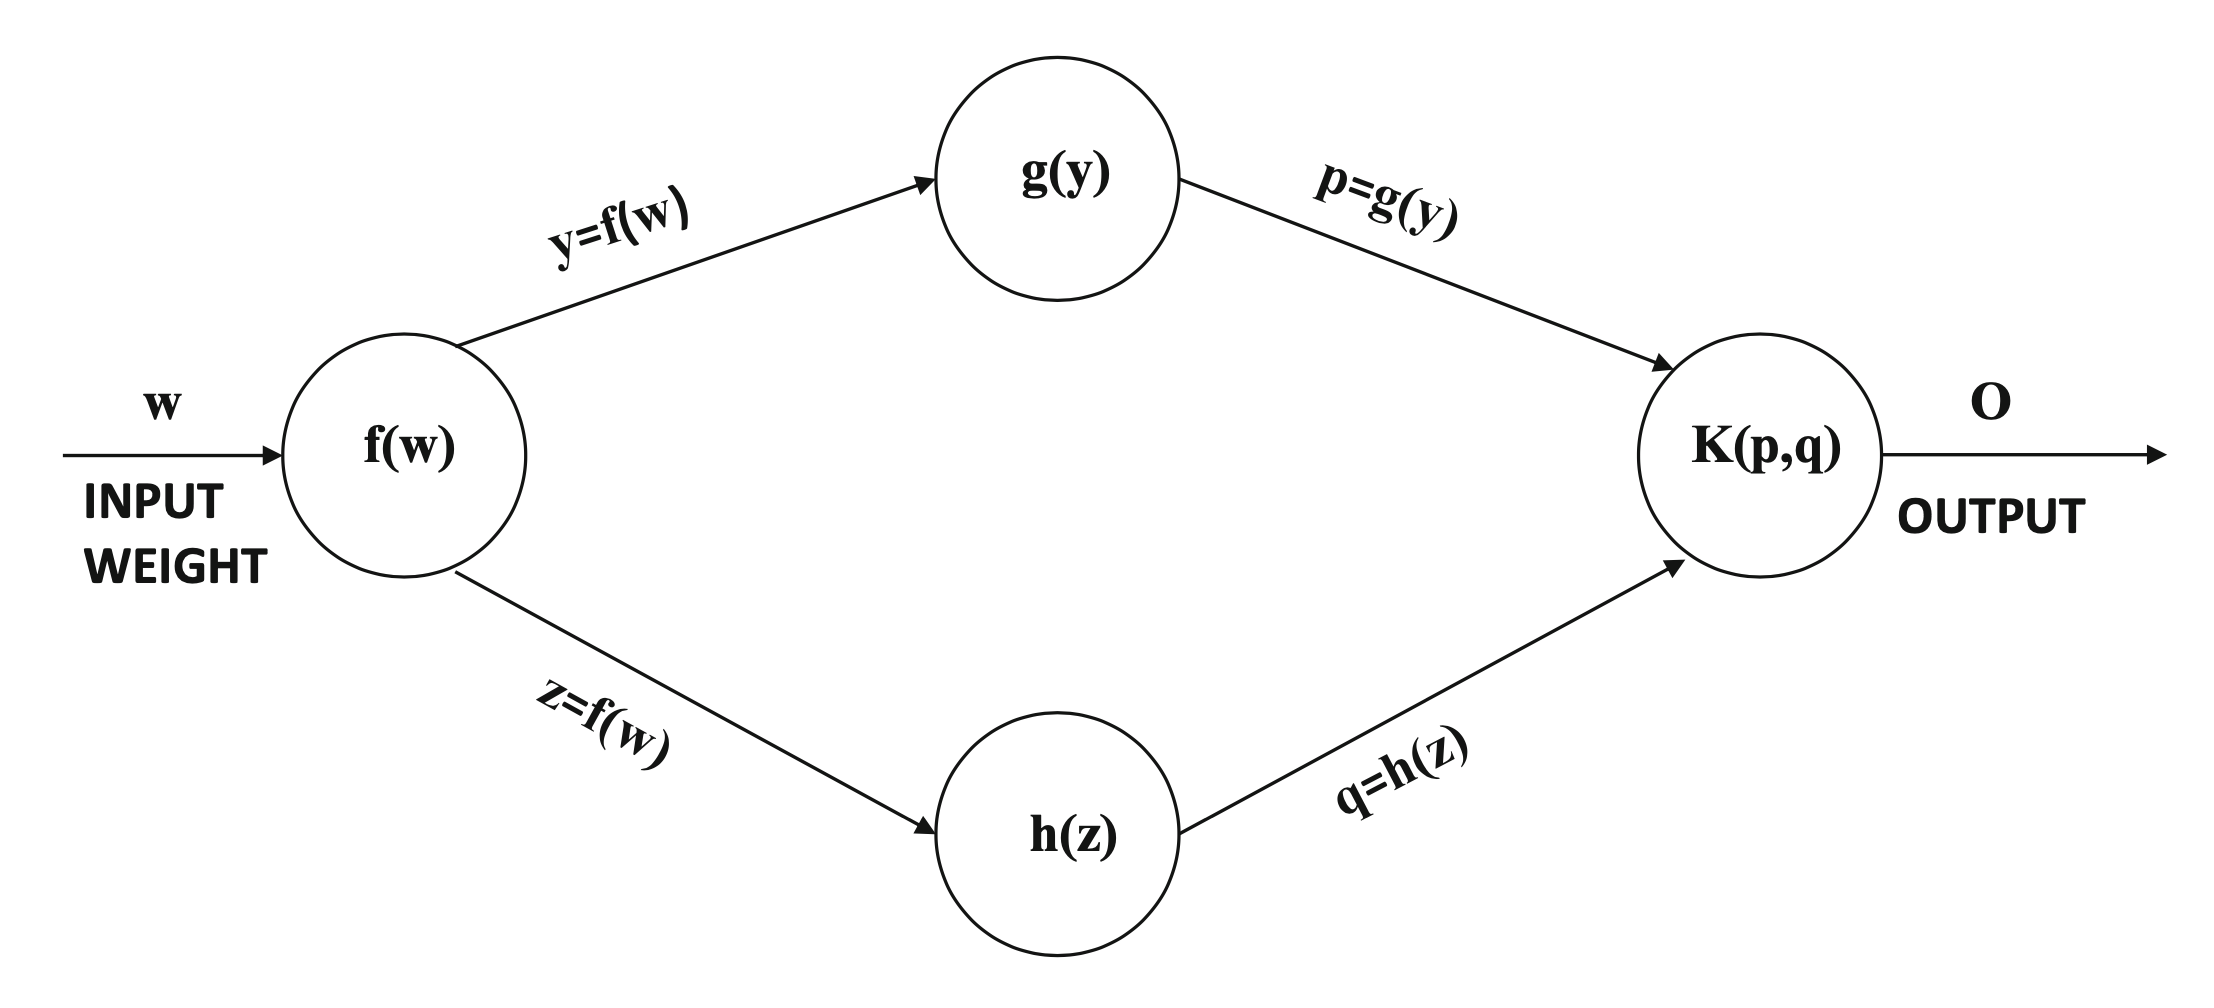
\includegraphics[width=11cm]{thesis/figures/neural-network-example-backprop-aggarwal-2018.png}
    \caption{Neural network with one input node, one hidden layer with two nodes and a single output layer (as illustrated by \cite[Figure 1.13]{Aggarwal18}).}
    \label{fig:neural-network-example-backprop}
\end{figure}

In this example, we are given a network with one input node (neuron), a hidden layer with two nodes and a single output layer with one node. The input to the network is denoted as $w$ and is the product of the input data and the weights in the input layer. The activation functions of the network are denoted as $f$, $g$ and $h$. Moreover, the results of the activation functions are denoted as $y$, $z$, $p$, $q$, and the function $K$ combines the result of $p$ and $q$ resulting in the output value $o$. We assume that the weights of the hidden layer is applied to the previous layer's output values during $g$ and $h$ and the weights of the output layer is applied at $K$. The forward pass in this network is pretty straight forward; we start the input node, pass the data on to $g$ and $h$ and combine the results in the output layer. Now, for the backwards pass we first need to compute the loss at the output node using a loss function $L$. Furthermore, we compute the derivative of $L$ with respect to the input value, $w$ in this case. More formally, we need to compute
\begin{align}
    \parder{L}{w}
    &= \parder{L}{o} \cdot \parder{o}{w} \\
    &= \parder{L}{o} \cdot \left[
    \parder{o}{p} \cdot \parder{p}{w} +
    \parder{o}{q} \cdot \parder{q}{w}
    \right] \text{(chain rule)} \\
    &= \parder{L}{o} \cdot \left[
    \parder{o}{p} \cdot \parder{p}{y} \cdot \parder{y}{w} + 
    \parder{o}{q} \cdot \parder{q}{z} \cdot \parder{z}{w}
    \right] \text{(chain rule)} \\
    &= \parder{L}{o} \cdot \left[
    \undertext{\parder{K(p, q)}{p} \cdot g'(y) \cdot f'(w)}{Path on top} + 
    \undertext{\parder{K(p, q)}{q} \cdot h'(z) \cdot f'(w)}{Path on bottom}
    \right]
\end{align}

With this example in mind, we have illustrated how the derivatives are being calculated for a small neural network. There exists, effective and more general frameworks to derive the derivative of the loss with respect to the input values, but we will leave those details out and kindly refer the reader to \cite[Chapter 1.3]{Aggarwal18} for more details.

We have now gone over the forward and backward passes, which are the first two steps of the so called backpropagation algorithm. The remaining step of the algorithm is now to use the computed derivatives to update the weights of the ANN. To do this, we use the gradient descent (GD) algorithm. The main idea of gradient descent is to update the weights iteratively by moving them in the opposite direction of the gradient (i.e. the steepest descent), and by doing so, we will hopefully reach some local minimum leading better to fitting weights for the input-output data. In standard gradient descent, we perform its steps in the following manner
\begin{align}
    W \Leftarrow W - \alpha \cdot \parder{L}{W}
\end{align}
where $W = \left( w_1, w_2, \ldots, w_d \right)$ is the matrix consisting of the $d$ weights of an ANN. The learning rate $\alpha$ is a hyperparameter and determines how much learning we want to do in each step. The learning rate is usually set to a relatively low value, in the order of $10^{-2}$ to $10^{-5}$.

Even though gradient descent works great for small applications, once we scale the number of parameters (weights) in the ANN to the more extremes (e.g. in the order of millions), it becomes impractical to compute for the entire training data at once. Furthermore, we observe that a loss function $L$ usually can be written as a sum of the loss of the individual training data points (denoted $L_i$ for $i$th training point), as shown in \cref{eqn:loss-function-sum-individual}.
\begin{align}
    \label{eqn:loss-function-sum-individual}
    L = \sumlim{i=1}{n} L_i
\end{align}
Using the observation that we are able to write the loss function as the sum in \cref{eqn:loss-function-sum-individual}, we introduce the stochastic gradient descent (SGD) method. Instead of performing gradient descent on the whole input data, SGD instead performs gradient descent for each input data separately, as shown in \cref{eqn:sgd}. We call it stochastic, because a random sample of the training data is chosen for each iteration.
\begin{align}
    \label{eqn:sgd}
    W \Leftarrow W - \alpha \cdot \parder{L_i}{W}
\end{align}
where $n$ is the number of input data points and $L_i$ represents the loss the $i$th input. An advantage SGD has over GD, is that it runs a lot faster, at the expense of greater loss. Thankfully, there exists a variant of SGD which seeks to find a balance between speed and loss, namely the mini-batch stochastic gradient descent. In mini-batch stochastic gradient descent, one uses a batch $B=\enclc{j_1, \ldots, j_m}$ of input training data indices when computing the weight updating, as shown in \cref{eqn:mbsgd}.
\begin{align}
    \label{eqn:mbsgd}
    W \Leftarrow W - \alpha \cdot \sumlim{j \in B}{} \parder{L_j}{W}
\end{align}
Mini-batch stochastic gradient descent often finds the best trade-off between stability, speed and memory requirements. It should be noted, however, that the memory requirement increases with the use of mini-batches, due to the fact that we have to store bigger matrices in memory during training. One typically chooses batch sizes that are power of 2 (e.g. 32, 64, 128 or 256), since most modern hardware architectures are optimized for it.

In addition to the different variants of gradient descent, there exist a bunch of other variants which can solve issues such as getting stuck in local minimas or speeding up the training process. We will not go into detail on all these strategies here, but kindly refer the reader to \cite[Chapter 3.5]{Aggarwal18} for more details.

\section{Clustering techniques}
In a supervised machine learning setting, one usually has some data $X$ and associated labels $y$. The task then is to train a model to predict labels $y$ given data $X$. In an unsupervised setting, however, the labels $y$ might not be present. To predict the labels $y$, clustering techniques are usually applied.

Clustering is one of the most important techniques in unsupervised machine learning. Clustering algorithms divides some data $X$ into clusters (groups) such that the data in each cluster are similar in some sense. An example of this is clustering by distance (e.g. euclidean). If we cluster by distance, we want the distance between any two data points belonging to the same cluster to be small. This distance is also referred to as the intracluster distance. Unfortunately, it is not enough to only minimize the intracluster distance, we also have to ensure that distance between the clusters is as large as possible. To measure the distance the distance between two clusters we measure the distance between two data points belonging to different clusters. The distance between clusters is called intercluster distance. If a clustering algorithm is able to create clusters such that we have small intracluster distance and large intercluster distance, it indicates that the cluster algorithm is good for the data at hand. We note, however, that data can be very complex and it can be very hard to find good clusters.

We will now go over some common clustering algorithms, explain how they work and discuss their strengths/weaknesses. In each of the clustering algorithms, we can assume that we are given some data $X = \enclc{x_1, x_2, \ldots, x_n} \in \R^{n \times d}$.

\subsection{k-means clustering}
The k-means clustering method \cite[Section 9.1]{bishop2006} is an unsupervised machine learning algorithm which is used to identify clusters in data. The algorithm uses an iterative approach to search for $k$ clusters, where $k$ is a pre-determined number of clusters (i.e. hyperparameter). There exists several variants of this algorithm and we will discuss two of them in later subsections (\cref{sec:mini-batch-k-means-clustering} and \cref{sec:k-medoids-clustering}). We will now explain the standard (and naïve) variant of the algorithm, which is usually referred to as Lloyd's algorithm.

The standard k-means clustering algorithm works as follows. The first step is to determine the initial cluster means, or centroids. Since we want the algorithm to output $k$ clusters, we have to decide $k$ initial centroids. The simplest way to do this is to select $k$ random data points to be the initial $k$ centroids. The next step is to calculate the euclidean distance between each data point to the cluster centroids. We do so because we want to determine which cluster each data point belong to. Furthermore, we assign each data point to its closest cluster centroid and compute the mean of each cluster. The third and final step is to move the cluster centroid to the newly computed mean of each cluster. The second and third step is then repeated until the desired clustering is achieved.

More formally, the goal of k-means clustering is to minimize the squared distance between the points in each cluster to its respective centroid. This is also referred to as the within-cluster sum of squares (WCSS). The objective is to find
\begin{align}
    \argmin_{C} \sumlim{i=1}{k} \sumlim{x \in C_i}{} \norm{x - \mu_i}^2
\end{align}
where $C = \enclc{C_1, C_2, \ldots, C_k}$ are the clusters of the data $X$, $k$ is the desired number of clusters and $\mu_i$ is the cluster centroid of cluster $C_i$.

The main advantage of k-means clustering is its simplicity, both in implementation and interpreting the results. The algorithm also scales well to larger data sets and there is only one hyperparameter to tune (number of clusters $k$). As for the disadvantages, the algorithm is rather sensitive to the initialization of centroids in the first step. If we were to select very bad initial centroids, the convergence time of the algorithm increases greatly and we might not even get good clusters. We also have to choose the number of clusters manually, which is a downside if we have no additional knowledge of the data beforehand. In addition to this, the algorithm (as with any distance-based clustering algorithm) suffers from the curse of dimensionality (\cref{fig:curse-of-dimensionality}), i.e., the fact that when the dimensionality increases it becomes more and more difficult to distinguish between data points (all points converge to the same distance).

\begin{figure}[H]
    \centering
    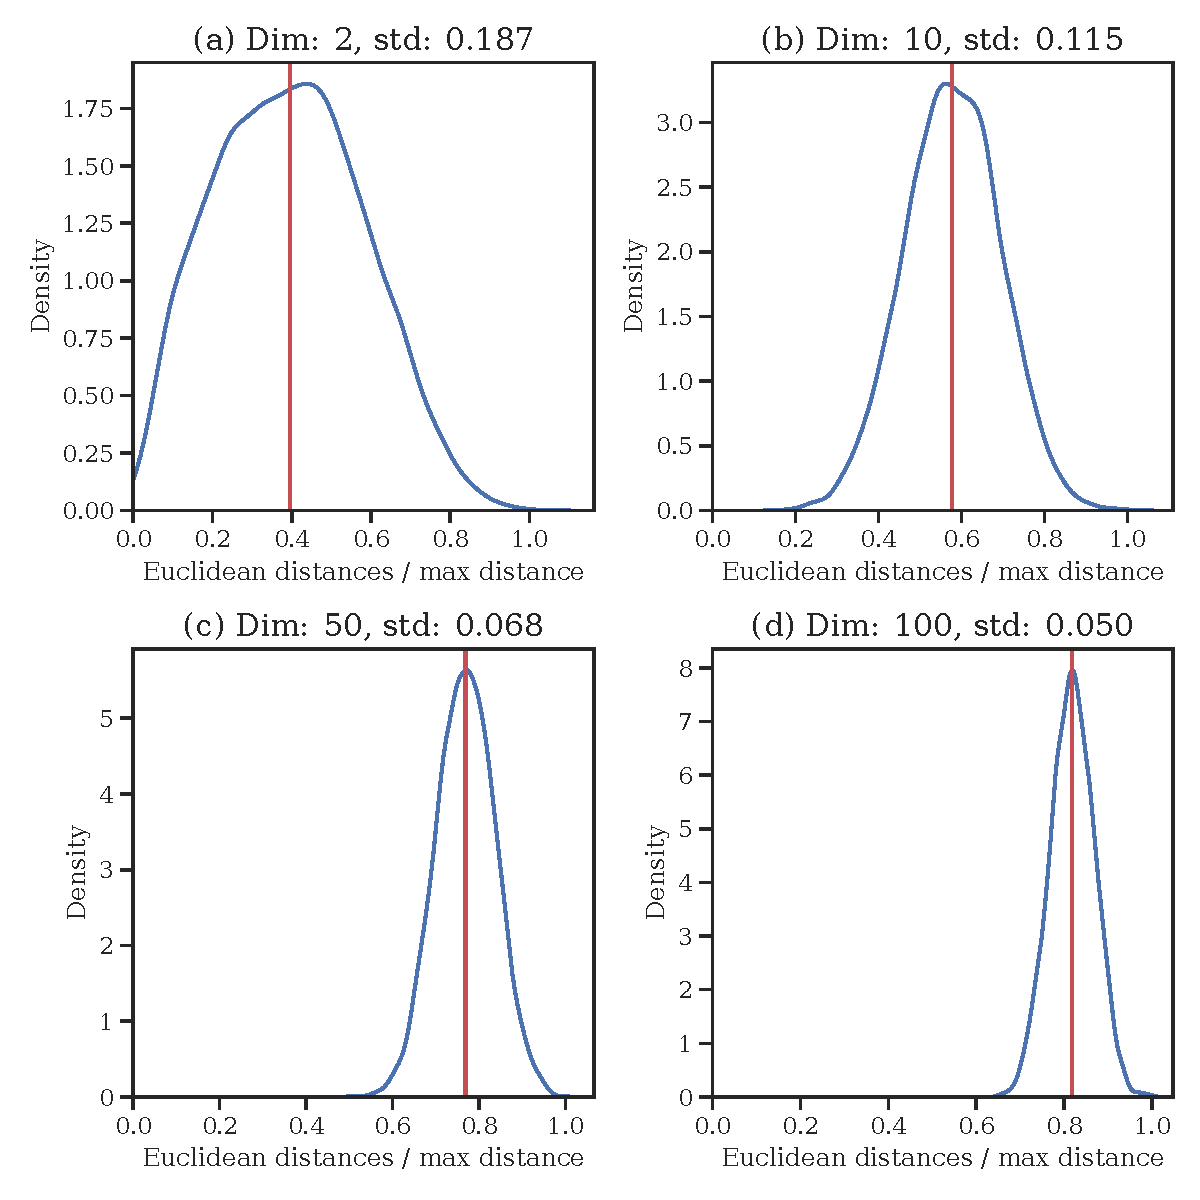
\includegraphics[width=0.7\textwidth]{thesis/figures/curse-of-dimensionality.pdf}
    \caption{Curse of dimensionality: the distance between points in higher dimensional spaces become the same as the dimensionality increases, and thus, it is harder to differentiate between points using distance metrics. The blue line represents the density of the pairwise euclidean distances (divided by max distance to normalize x-axis). The red line is the mean distance.}
    \label{fig:curse-of-dimensionality}
\end{figure}

\textbf{TODO: Write cons/pros.}

\subsection{Mini-batch k-means clustering}
\label{sec:mini-batch-k-means-clustering}
The time it takes for K-means clustering to converge strongly depends on the number of data points $n$ and the desired number of clusters $k$. In order to reduce the computation time, mini-batch k-means clustering was introduced \cite{sculley2010}. The mini-batches are randomly sampled subsets of the training data for each training iteration (similar to the mini-batches in gradient descent). By using mini-batches, we drastically reduce the computational requirement required to converge to a local solution and, as noted by the authors in \cite{sculley2010}, the results of mini-batch k-means clustering tend to only be slightly worse than the standard algorithm.

The algorithm is very similar to the standard k-means clustering algorithm and comprises two major steps. In the first step, we initialize $k$ cluster centroids and sample $B=\enclc{b_1, b_2, \ldots, b_m} \subset X$ points at random from the data set $X$, where $m$ is the mini-batch size. In the second step, we update the cluster centroids by gradually moving the centroids. For each sample $b$ in the mini-batch, the centroids are updated by taking the average of $b$ and the previous points assigned to the centroid. By doing so, the centroid is moved with a decreasing rate over time. The first and the second step is repeated until convergence is met.

\textbf{TODO: Write cons/pros.}

\subsection{K-medoids clustering}
\label{sec:k-medoids-clustering}
K-medoids clustering was introduced as an alternative to the standard K-means clustering algorithm \cites{Kaufman1990}[p. 427 - 428]{bishop2006}. K-medoids clustering uses data points for its cluster centroids and works with any dissimilarity measures, making it more interpretable and robust to outliers than K-means clustering. A medoid of a cluster is a data point where the average dissimilarity between the medoid itself and all other data points in the same cluster is being minimized \cite{Kaufman1990}.

To solve the k-medoids problem efficiently, the Partitioning Around Medoids (PAM) algorithm is often used. Similar to the standard K-means clustering algorithm, PAM consists of two main stages called build and swap. In the build stage, we greedily select $k$ of the $n$ data points to be the initial cluster medoids, denoted $M = \enclc{m_1, m_2, \ldots, m_k} \subset X$. To select $M$ initially, we want to minimize the dissimilarity between the cluster medoids and associated points in the cluster. In other words, initially we set the first medoid $m_1$ to be the data point such that the dissimilarity between then medoid and all other data points is minimized. Then, for all proceeding medoids ($m_2, \ldots, m_k$), we look for medoids such that the dissimilarity between the additional medoid, the data points associated with the new medoid and all other medoids (and its associated data points) is minimized. This process is repeated until we have $k$ medoids. Following, the swap stage consists of iteratively swapping out the $k$ medoids with other data points from the data set, if it minimizes the overall dissimilarity. The algorithm terminates if by swapping the medoids with other data points we do not get lower dissimilarity.

Even though K-medoids clustering seems to be the superior choice over K-means clustering, it suffers from the fact it is more computationally heavy to compute and thus is not always feasible to run for large data sets.

\textbf{TODO: Write cons/pros.}

\subsection{Gaussian mixture models (GMMs)}
\label{sec:gmm-clustering}
Gaussian mixture models (GMMs) are probability distributions which consists of a mixture of multiple Gaussians \cite[Section 9.2]{bishop2006}. A Gaussian (also called normal) is a probability distribution which was several nice properties, such as mean as its mode and symmetry. In the context of cluster algorithms, GMMs can be used to cluster data points by using multivariate (i.e. of higher dimension) Gaussian distributions as cluster centroids. In particular, for each cluster centroid $c_i, 1 \leq i \leq k$, we define $\mu_i$ to be the cluster mean, $\Sigma_i$ to be the cluster covariances and $\pi_i$ to be the mixing coefficients. The cluster mean $\mu_i$ and covariances $\Sigma_i$ determines the localization and spread for each cluster, while the mixing coefficients $\pi_i$ determine how much we emphasize each cluster. In other words, by using Gaussian distributions, we get more freedom as to how the clusters are shaped and how much to prioritize them for each data point. To estimate the parameters $\theta = \enclc{\mu, \Sigma, \pi}$ of GMMs, the Expectation-Maximization (EM) algorithm is often used and is an iterative algorithm.

The EM algorithm starts off my initializing its parameters $\mu$, $\Sigma$ and $\pi$. There exists several methods for initializing the parameters and it is common to first run K-means clustering on the data in order to obtain a suitable starting point. By running K-means clustering first, the parameters are computed by using statistics from the result of K-means. Furthermore, the EM algorithm consists of two main stages, namely expectation and maximization. In the expectation stage compute the responsibilities for each data point in $X$ using the current set of parameters. With responsibilities, we mean how much each Gaussian is responsible for explaining a single data point in $X$. Next, in the maximization step, the responsibilities from the expectation step is used to update the parameters such that the likelihood $\text{P}(X | \theta)$ is maximized. The likelihood $\text{P}(X | \theta)$ tells us how good the set of parameters $\theta$ fits our data $X$. The exact derivation and update rules for each parameter is left out and we refer the reader to \cites[Section 9.4]{bishop2006} for more details. Once a suitable threshold is met with respect to $\text{P}(X | \theta)$, the algorithm terminates and we have converged to a set or parameters $\hat{\theta}$. Using the final parameters, $\hat{\theta}$ we predict which Gaussian (i.e. cluster) each data point in $X$ is associated with.

\textbf{TODO: Write cons/pros.}

\subsection{Hierarchical clustering}
Hierarchical clustering is a group of clustering algorithms which constructs clusters by recursively partitioning the data points of $X$ in top-down or bottom-up fashion \cite{Rokach2005}. These two methods are divided into what we call agglomerative- and divisive hierarchical clustering. Using agglomerative hierarchical clustering, each data point in $X$ starts off in their own cluster and are successively merged until all points are merged into a single cluster. In contrast to the agglomerative method, divisive hierarchical clustering starts off with all data points in $X$ in a single cluster. Then, the single cluster is divided into smaller clusters, until each point is in its own cluster. The output of an hierarchical clustering algorithm is a dendrogram, which represents the nested clustering structure. An example of a dendrogram is illustrated in \cref{fig:dendrogram-example}.
\begin{figure}[H]
    \centering
    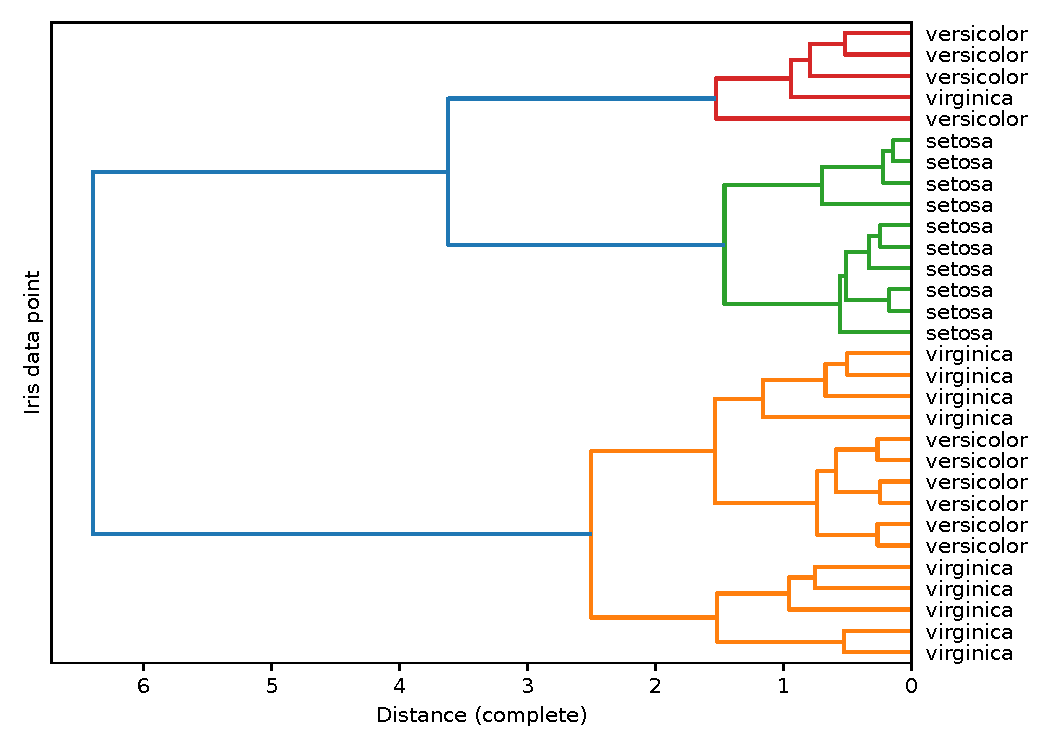
\includegraphics[width=0.9\textwidth]{thesis/figures/dendrogram-example.pdf}
    \caption{Example of a dendrogram plot using the Iris dataset \cite{Fisher1936}.}
    \label{fig:dendrogram-example}
\end{figure}

To merge or divide clusters, we use some similarity measure in order to either merge similar data points (agglomerative) or divide dissimilar data points (divisive). Exactly which data points we choose to merge or divide depends on which criterion we want to optimize. There exist several different criterions one may choose to perform hierarchical clustering. Below we will list some of the most common ones and very briefly discuss the pros/cons for each criterion.
\begin{itemize}
    \item \textbf{Single-linkage clustering} --- combines two clusters that contain the closest pair (i.e. largest similarity) of elements that do not yet belong to the same cluster as each other.
    \begin{itemize}
        \item Single-linkage clustering tends to produce clusters of long chains, which can lead to the clustering of data points which in reality are far apart from each other.
        \item Single-linkage clustering is fast to use for big data sets and is able to create clusters of different shapes and sizes.
        \item Single-linkage clustering is sensible to noise.
    \end{itemize}
    \item \textbf{Complete-linkage clustering}  --- combines two clusters that contain the furthest pair (i.e. smallest similarity) of elements that do not yet belong to the same cluster as each other.
    \begin{itemize}
        \item Complete-linkage clustering is biased towards spherical clusters.
        \item Complete-linkage clustering works well on data with noise.
        \item Complete-linkage clustering tends to split large clusters.
    \end{itemize}
    \item \textbf{Average-linkage clustering} --- combines two clusters such that the average pairwise distance within the newly created cluster is minimum.
    \begin{itemize}
        \item Average-linkage clustering is biased towards spherical clusters.
        \item Average-linkage clustering works well on data with noise.
    \end{itemize}
    \item \textbf{Ward-linkage clustering} --- combines two clusters such that the variance of the newly created cluster is minimum \cite{Ward1963}.
    \begin{itemize}
        \item Ward-linkage clustering is biased towards spherical clusters.
        \item Ward-linkage clustering works well on data with noise.
    \end{itemize}
\end{itemize}

\textbf{TODO: Write cons/pros.}

\subsection{Spectral clustering}
Spectral clustering is a clustering algorithm which uses the eigenvalues of the affinity matrix (e.g. a similarity matrix using pairwise euclidean distances) of the data $X$ to reduce the dimensionality of the data, before applying some common clustering algorithm, such as K-means clustering \cite{Andrew2002}.

Imagine that we want to cluster the data into $k$ clusters. Spectral clustering starts off with the construction of the affinity matrix $A$. Typically, one uses some similarity measure to create pairwise distances between data points to create such an affinity matrix. Then, the graph Laplacian $L = D - A$ is computed, where $D$ is a diagonal matrix with $D_{ii} = \sumlim{j}{} A_{ij}$ and $A$ is the affinity matrix. The graph Laplacian $L$ is simply a matrix representation of a graph, and in our case, the similarities between data points in $X$. Next, the eigenvectors of $L$ is computed, and using these eigenvectors, we now have a lower-dimensional space of the original data $X$ (from $d$ dimensions to $k$). Lastly, we use a clustering algorithm, such as K-means clustering, on the eigenvectors of $L$ to get the final clustering.

\textbf{TODO: Write cons/pros.}

\subsection{HDBSCAN}
Clusters come in different shapes and sizes, and real-life data is rather noisy. DBSCAN is a density-based algorithm invented to cope with such problems \cite{Ester1996}. It, however, is only able to produce a "flat" clustering given some global threshold parameter. HDBSCAN is a generalization of DBSCAN and improves on it by creating a complete density-based clustering hierarchy \cite{Campello2013}, automatically extracting flat clusters. HDBSCAN is different from the other clustering algorithms we have seen so far, as it is able to create clustering without predetermining the number of clusters beforehand and can mark data points a noise. To fully understand the HDBSCAN algorithm, we will introduce its key concepts and then explain how the algorithm works in practice.

HDBSCAN is a density-based clustering algorithm and, for this reason, requires an inexpensive density estimation method to be efficient. Using k-nearest neighbours, the authors of HDBSCAN is able to estimate the density in an efficient manner. In particular, they define the \textbf{core distance} of a data point $x \in X$ to be the distance to the $\textit{minPts}$-nearest neighbour (including $x$), denoted $d_{core}(x)$. $\textit{minPts}$ is a hyperparameter and controls how conservative we want the clustering to be; the larger $\textit{minPts}$, the more points will be marked as "noise". To further spread apart data points that have low density, the \textbf{mutual reachability distance} metric (MRD) is defined, as seen in \cref{eqn:mutual_reachability_distance}.
\begin{align}
    d_{mreach}(x, y) = \max \enclc{ d_{core}(x), d_{core}(y), d(x, y) }
    \label{eqn:mutual_reachability_distance}
\end{align}
where $d(x, y)$ is the distance between data point $x$ and data point $y$ using the original distance metric. Under the MRD metric, data points in dense regions will not change their distances, but sparser data points will be pushed away such that the distance is at least their core distance to other points.

Next, given the MRD metric, we use it to find dense areas in the data. To find such areas, we create a minimal spanning tree (MST) where each node represents a data point $x \in X$ and edges connecting pairs of nodes is weighted by the MRD between the two nodes. By using an MST, we get a graph with the minimal set of edges between nodes such that the weight between the nodes is minimized. Also, by dropping one edge, we graph becomes disconnected, i.e., each pair of nodes is connected by exactly one edge. Using these two facts, we can create a clustering hierarchy in a single-linkage clustering manner. First, the weights of the edges of the MST is sorted in increasing order. Following, we iterate over the sorted edges of the MST and merge data points into clusters (note that each individual data point is its own cluster initially). Now, from the hierarchical clustering we are left with a dendrogram, similar to the one from \cref{fig:dendrogram-example}, but are left with a critical question; how should we define the cut in order to get a flat clustering?

Dendrograms can be very difficult to interpret once a certain number of data points is reached. For this reason, the authors of HDBSCAN condense (or compact) the dendrogram from the hierarchical clustering such that a flat clustering can be obtained rather easily. First, the notion of \textbf{minimum cluster size} is defined and is a hyperparameter controlling the minimal cluster size at any time. Following, we walk down the dendrogram, starting from the root cluster, and at each split we check whether or not the new cluster created by the split has at least \textbf{minimum cluster size} data points in them. If the new cluster has at least \textbf{minimum cluster size} data points in them, we let that cluster be in the tree. If the new cluster has less than the \textbf{minimum cluster size}, then we let the parent cluster identify the new cluster and the node is removed from the tree. As we walk through the dendrogram in order to condense it, we also include at what distance clusters merge into the parent cluster, i.e., "fall out of clusters". An example of a condensed diagram is down in \textbf{TODO}.

Now, to define the flat cut in the condensed diagram, we select the clusters such that the largest total area of "ink" is maximized, under an additional constraint that we can not select clusters that are descendants of an already selected cluster. Any clusters which are not selected are marked as noise, as they are merely artifacts of the initial hierarchical clustering. The final clustering is then decided, as illustrated from the example in \textbf{TODO}.

\textbf{TODO: Write cons/pros.}

\section{Dimensionality reduction techniques}
TODO 

\subsection{Principal Component Analysis (PCA)}
TODO

\subsection{Uniform Manifold Approximation and Projection (UMAP)}
TODO
